% !TeX root = ../tfg.tex
% !TeX encoding = utf8

\chapter{Apéndice}\label{ap:apendiceC}

En este apéndice se presentan dos experimentos relacionados con el uso de diferentes tamaños de lote y tasas de aprendizaje para un modelo que exhibe el doble descenso. Para ello, se empleará la arquitectura $2$NN sobre el subconjunto MNIST[$4000/1000$], al cual se le añadirá un porcentaje variable de ruido, y donde se utilizarán distintas tasas de aprendizaje con el optimizador Adam.\newline
 
\subsection*{Double descent con distinto tamaño de batch}

\begin{figure}[h!]
    \centering
    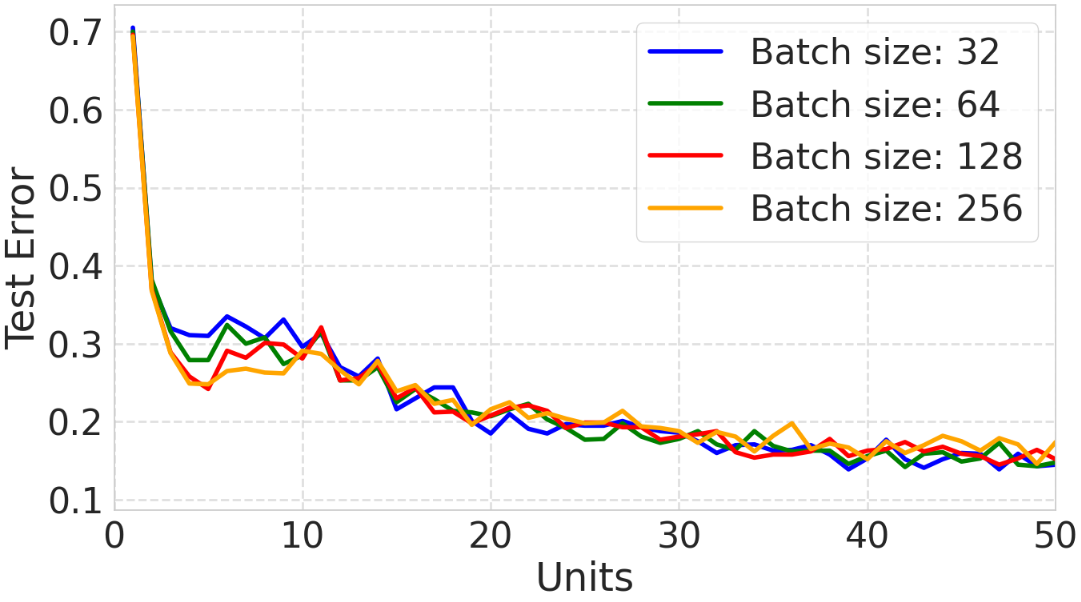
\includegraphics[width=0.5\textwidth]{img/experiments/batch_sizes_ddd.png}
    \caption[Doble descenso para distintos tamaños de lote.]{Error en test respecto a distintas configuraciones de tamaño de lote obtenido por la red $2$NN sobre el subconjunto MNIST[$4000/1000$] con $10$\% de ruido agregado.}\label{fig:dddbatchsizes}
\end{figure}

En la Figura~\ref{fig:dddbatchsizes} se observa que, para distintas configuraciones de tamaño de batch, se manifiesta el doble descenso, siendo más notable al utilizar tamaños de batch mayores. Por otro lado, la Tabla~\ref{tab:dddbatchsizes} muestra que, al incrementar el tamaño de batch, el tiempo de entrenamiento disminuye, lo cual es lógico, ya que se procesan un mayor número de ejemplos en cada iteración.\newline

Por tanto, considerando ambos resultados, se concluye que utilizar un tamaño de batch elevado ($128$ o $256$) es la opción más adecuada para los distintos experimentos a realizar, ya que permite observar el fenómeno de forma más clara y con menor coste computacional.\newline

\begin{table}[h!]
    \centering
    \begin{tabular}{|c|c|c|c|}
    \hline
    \textbf{Modelo}       & \textbf{Dataset} & \textbf{Batch size} & \textbf{Entrenamiento} \\ 
    \hline
    $2$NN ($1-50$)     & MNIST[$4000/1000 - 10$\% noise]      & $32$      & $15$h $2$min         \\ 
    $2$NN ($1-50$)     & MNIST[$4000/1000 - 10$\% noise]      & $64$      & $11$h $56$min         \\ 
    $2$NN ($1-50$)     & MNIST[$4000/1000 - 10$\% noise]      & $128$      & $11$h $14$min         \\ 
    $2$NN ($1-50$)     & MNIST[$4000/1000 - 10$\% noise]      & $256$      & $10$h $23$min         \\
    \hline
    \end{tabular}
    \caption[Resumen de los experimentos realizados para el doble descenso con distinto tamaño de lote.]{Resumen de los experimentos realizados para el doble descenso con distinto tamaño de lote.}\label{tab:dddbatchsizes}
\end{table}

\subsection*{Double descent con distinto learning rate}

\begin{figure}[h!]
    \centering
    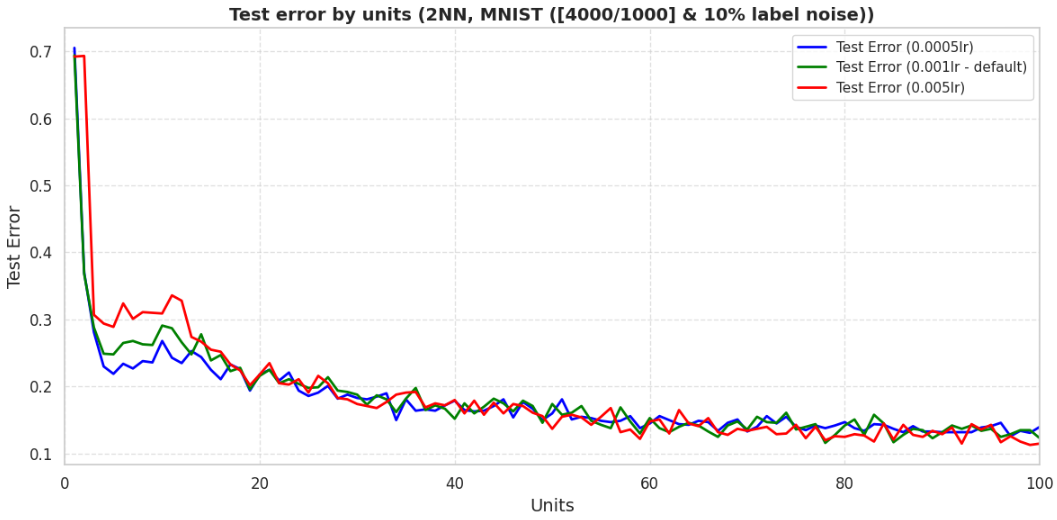
\includegraphics[width=0.5\textwidth]{img/experiments/learning_rates_ddd.png}
    \caption[Doble descenso para distintas tasas de aprendizaje.]{Error en test respecto a distintas configuraciones de tasa de aprendizaje obtenido por la red $2$NN sobre el subconjunto MNIST[$4000/1000$] con $10$\% de ruido agregado.}
    \label{fig:difflr}
\end{figure}

En la Figura~\ref{fig:difflr} podemos observar cómo se manifiesta el doble descenso para distintas configuraciones de la tasa de aprendizaje. En particular, el ``pico'' del error de test se hace más pronunciado a medida que la tasa de aprendizaje aumenta, dado que para una tasa igual a $5 \times 10^{-4}$, el máximo error en test es mayor que para el valor por defecto de la tasa de aprendizaje ($10^{-4}$), y este, a su vez, es mayor que para la mínima tasa de aprendizaje utilizada ($5 \times 10^{-5}$).\newline

En conclusión, esto nos indica que, si un modelo presenta el doble descenso, no es necesario preocuparse en exceso por ajustar de manera fina la tasa de aprendizaje, puesto que, dentro de ciertos rangos de valores para dicha tasa de aprendizaje, el modelo sigue manifestando el suceso, lo que indica que el uso por defecto de la tasa de aprendizaje resulta ser suficiente.\newline

Finalmente, para concluir esta subsección se muestra en la Tabla~\ref{tab:difflr} un resumen de los experimentos realizados junto con sus respectivos tiempos de entrenamiento.\newline

\begin{table}[h!]
    \centering
    \begin{tabular}{|c|c|c|c|}
    \hline
    \textbf{Modelo}       & \textbf{Dataset} & \textbf{Tasa aprendizaje} & \textbf{Entrenamiento} \\ 
    \hline
    $2$NN ($1-100$)     & MNIST[$4000/1000 - 10$\% noise]      & $0.005$      & $23$h $53$min         \\ 
    $2$NN ($1-100$)     & MNIST[$4000/1000 - 10$\% noise]      & $0.001$ (default)      & $26$h $50$min     \\ 
    $2$NN ($1-100$)     & MNIST[$4000/1000 - 10$\% noise]      & $0.0005$      & $27$h $32$min         \\ 
    \hline
    \end{tabular}
    \caption[Resumen de los experimentos realizados para el doble descenso con distintas tasas de aprendizaje.]{Resumen de los experimentos realizados para el doble descenso con distintas tasas de aprendizaje.}\label{tab:difflr}
\end{table}

\endinput
%------------------------------------------------------------------------------------
% FIN DEL APÉNDICE. 
%------------------------------------------------------------------------------------
